% !TeX spellcheck = en_US

\documentclass[main.tex]{subfiles}

\begin{document}
    \subsection{Motivation and Relevancy}
    
    \begin{frame}{The Most Sexiest Job on Earth}
        \begin{columns}
            \begin{column}{.6\textwidth}
                \begin{justify}
                    \textit{"I keep saying \textbf{the sexy job in the next ten years will be statisticians}. People think I’m joking, but who would’ve guessed that computer engineers would’ve been the sexy job of the 1990s? \textbf{The ability to take data—to be able to understand it, to process it, to extract value from it, to visualize it, to communicate it—that’s going to be a hugely important skill in the next decades}, not only at the professional level but even at the educational level for elementary school kids, for high school kids, for college kids. Because now we really do have essentially \textbf{free and ubiquitous data}. So the complimentary \textbf{scarce factor is the ability to understand that data and extract value from it}."}
                    \vspace*{1mm}
                    
                    Hal Varian, Google Chief Economist, 2009
                \end{justify}
            \end{column}
            \begin{column}{.4\textwidth}
                \begin{figure}
                    \label{fig:hal-varian}
                    \includegraphics[width=.6\textwidth,cframe=gray]{figures/external/hal-varian.jpg}
                \end{figure}
            \end{column}
        \end{columns}
    \end{frame}

    \begin{frame}{The Oil of the 21st Century}
        \begin{columns}
            \begin{column}{.5\textwidth}
                \begin{figure}
                    \label{fig:internet-usage-1}
                    \includegraphics[width=\textwidth,cframe=gray]{figures/external/internet-usage-1.png}
                    
                    \tiny{\textbf{\href{https://de.statista.com/statistik/daten/studie/169455/umfrage/prognose-zum-weltweiten-datenvolumen-nach-segmenten/}{SOURCE}}}
                \end{figure}
            \end{column}
            \begin{column}{.5\textwidth}
                \begin{figure}
                    \label{fig:internet-usage-2}
                    \includegraphics[width=\textwidth,cframe=gray]{figures/external/internet-usage-2.png}
                    
                    \tiny{\textbf{\href{https://deviq.io/resources/articles/feeling-overwhelmed-by-a-deluge-of-iot-data-iot-data-analytics-dashboards-can-help/}{SOURCE}}}
                \end{figure}
            \end{column}
        \end{columns}
        
        \begin{center}
            \textit{"Information is the oil of the 21st century, and analytics is the combustion engine."} – Peter Sondergaard, former senior vice president and global head of Research at Gartner, Inc, 1965
        \end{center}
    \end{frame}
    
    \begin{frame}{Labor Market Relevancy and Salary}
        \begin{columns}
            \begin{column}{.5\textwidth}
                \begin{figure}
                    \label{fig:job-openings}
                    \includegraphics[width=\textwidth,cframe=gray]{figures/external/job-openings.png}
                    
                    \tiny{\textbf{\href{https://media.thinknum.com/articles/massive-increase-in-demand-for-data-science-jobs-in-2019/}{SOURCE}}}
                \end{figure}
            \end{column}
            \begin{column}{.5\textwidth}
                \begin{figure}
                    \label{fig:salary}
                    \includegraphics[width=\textwidth,cframe=gray]{figures/external/salary.jpg}
                    
                    \tiny{\textbf{\href{https://www.datacareer.de/blog/data-scientist-salaries-in-europe-in-2018/}{SOURCE}}}
                \end{figure}
            \end{column}
        \end{columns}
    
        \begin{center}
            While structured data continues to \textbf{quantitatively remain static or decrease}, \textbf{unstructured data is increasingly rapidly}. That means that \textbf{companies must deal with this data} and may even gain a \textbf{competitive advantage} from it. Many companies have already recognised this trend and are eagerly looking for "data scientists" and many have already specifically developed a data science programme. The \textbf{demand in this field is already large and will increase} just as rapidly as unstructured data.
        \end{center}
    \end{frame}
    
    \subsection{Real-World Examples}
    
    \begin{frame}{Demand Forecasting}
        \begin{columns}
            \begin{column}{.6\textwidth}
                \begin{justify}
                    \textit{"\textbf{Otto} went further and created a system using the technology of Blue Yonder, a startup in which it holds a stake. A \textbf{deep-learning algorithm}, which was originally \textbf{designed for particle-physics experiments at the CERN laboratory} in Geneva, does the heavy lifting. It analyses around \textbf{3bn past transactions and 200 variables} (such as past sales, searches on Otto’s site and weather information) to \textbf{predict what customers will buy a week before they order}. The AI system has proved so reliable—it \textbf{predicts with 90\% accuracy} what will be sold within 30 days—that Otto allows it \textbf{automatically to purchase around 200,000 items a month} from third-party brands \textbf{with no human intervention}."}
                    \vspace*{1mm}
                    
                    The Economist, \href{https://www.economist.com/business/2017/04/12/how-germanys-otto-uses-artificial-intelligence}{How Germany’s Otto uses artificial intelligence}, 2017
                \end{justify}
            \end{column}
            \begin{column}{.4\textwidth}
                \begin{figure}
                    \label{fig:otto-blue-yonder}
                    \includegraphics[width=.8\textwidth]{figures/external/otto-blue-yonder.png}
                \end{figure}
            \end{column}
        \end{columns}
    \end{frame}
    
    \stepcounter{openexercise}
    \begin{frame}{Open Exercise \arabic{openexercise}}
        What do you think has been the major business problem here for Otto and what other problems concerning the corporate social responsibility have been solved but also have been evolved in the same step? 
        \note{
        According to The Economist: \textit{"Overall, the surplus stock that Otto must hold has declined by a fifth. The new AI system has \textbf{reduced product returns by more than 2m items a year}. Customers get their items sooner, which improves retention over time, and the technology also benefits the environment, because fewer packages get dispatched to begin with, or sent back."}
        
        }
    \end{frame}
    
    \begin{frame}{Product Recommender I/II}
        \begin{columns}
            \begin{column}{.6\textwidth}
                \begin{justify}
                    \textit{"In October 2006, Netflix [...] announced "The Netflix Prize" [...]. The mission: Make the company's \textbf{recommendation engine 10\% more accurate} -- or die coding. [...] And while a \textbf{million dollars} created attention, it was the data set -- over \textbf{100 million ratings of 17,770 movies from 480,189 customers} -- that had number-crunching nuts salivating. [...] What made the contest so hard? For one thing, the \textbf{sheer range of the data}: Some users in the set had only reviewed 9 movies, which was the minimum to be included, and gave the contestants very little information to get a good read on their tastes. On the other hand, some Netflix obsessives -- you know the type -- had rated over 900 films."}
                    \vspace*{1mm}
                    
                    Thrillist, \href{https://www.thrillist.com/entertainment/nation/the-netflix-prize}{The Netflix Prize: How a \$1 Million Contest Changed Binge-Watching Forever}, 2017
                \end{justify}
            \end{column}
            \begin{column}{.4\textwidth}
                \begin{figure}
                    \label{fig:netflix-prize}
                    \includegraphics[width=\textwidth]{figures/external/netflix-prize.jpg}
                \end{figure}
            \end{column}
        \end{columns}
    \end{frame}
    
    \stepcounter{openexercise}
    \begin{frame}{Open Exercise \arabic{openexercise}}
    Why is the ability to recommend products an important digital asset for companies in general and why is it for Netflix if the only product they offer is a subscription? 
    \note{
    \textbf{Up-selling and cross-selling} products of course \textbf{increases the revenues} of companies. The better the recommendations, the higher is the probability of customers to converse. Netflix can indeed up-sell but not cross-sell. As a subscription service, each new month gives every Netflix users a chance to \textbf{cancel the service}. Like all subscription companies, the best step Netflix can take to reduce churn is to create a great product that people are willing to pay for. Strong recommendations \textbf{increase the average watch time among viewers}, thus keeping the clip at which Netflix loses subscribers — known as its \textbf{churn rate} — as low as possible.
    
    }
    \end{frame}
    
    \begin{frame}{Product Recommender II/II}
        \begin{columns}
            \begin{column}{.6\textwidth}
                \begin{justify}
                    \textit{"At root, the retail giant’s recommendation system is based on a number of simple elements: \textbf{what a user has bought in the past, which items they have in their virtual shopping cart, items they’ve rated and liked, and what other customers have viewed and purchased}. Amazon (AMZN) calls this homegrown math “\textbf{item-to-item collaborative filtering},” and it’s used this algorithm to heavily customize the browsing experience for returning customers."}
                    \vspace*{1mm}
                    
                    Forbes, \href{https://fortune.com/2012/07/30/amazons-recommendation-secret/}{Amazon’s recommendation secret}, 2012
                    \\~\\                    
                    \textit{"Already, \textbf{35 percent} of what consumers purchase on Amazon and \textbf{75 percent} of what they watch on Netflix come from \textbf{product recommendations} based on such algorithms."}
                    \vspace*{1mm}
                    
                    McKinsey, \href{https://www.mckinsey.com/industries/retail/our-insights/how-retailers-can-keep-up-with-consumers}{How retailers can keep up with consumers}, 2013
                \end{justify}
            \end{column}
            \begin{column}{.4\textwidth}
                \begin{figure}
                    \label{fig:amazon-recommendation}
                    \includegraphics[width=\textwidth, cframe=gray]{figures/external/amazon-recommendations.png}
                \end{figure}
            \end{column}
        \end{columns}
    \end{frame}
    
    \begin{frame}{Personalization}
        \begin{columns}
            \begin{column}{.6\textwidth}
                \begin{justify}
                    \textit{"\textbf{How do we convince you that a title is worth watching?} Answering these questions is critical in helping our members discover great content, especially for unfamiliar titles. One avenue to address this challenge is to consider the artwork or imagery we use to portray the titles. \textbf{If the artwork representing a title captures something compelling to you, then it acts as a gateway into that title and gives you some visual “evidence” for why the title might be good for you}. The artwork may highlight an actor that you recognize, capture an exciting moment like a car chase, or contain a dramatic scene that conveys the essence of a movie or TV show. \textbf{If we present that perfect image on your homepage (and as they say: an image is worth a thousand words), then maybe, just maybe, you will give it a try}."}
                    \vspace*{1mm}
                    
                    Netflix Technology Blog, \href{https://medium.com/netflix-techblog/artwork-personalization-c589f074ad76}{Artwork Personalization at Netflix}, 2017
                \end{justify}
            \end{column}
            \begin{column}{.4\textwidth}
                \begin{figure}
                    \label{fig:netflix-personalization}
                    \includegraphics[width=\textwidth]{figures/external/netflix-personalization.png}
                \end{figure}
            \end{column}
        \end{columns}
    \end{frame}
    
    \begin{frame}{Predictive Maintenance}
        \begin{columns}
            \begin{column}{.6\textwidth}
                \begin{justify}
                    \textit{"Few sectors generate more data than the energy industry. But for years, oil giant \textbf{Shell} didn't know where parts were in its various facilities around the world; \textbf{it didn’t know when to restock; and it didn't know when maintenance issues were occurring until parts began failing}. With \textbf{machine downtime costing industrial companies millions of dollars a day}, Shell decided to harvest data to head off these issues. [...] Shell built an analytics platform [...] to run predictive models to \textbf{anticipate when more than 3,000 different oil drilling machine parts might fail} [...]. The tool [...] has helped Shell \textbf{reduced inventory analysis from over 48 hours to less than 45 minutes, shaving millions of dollars a year off the cost of moving and reallocating inventory}."}
                    \vspace*{1mm}
                    
                    Clint Boulton, \href{https://medium.com/netflix-techblog/artwork-personalization-c589f074ad76}{10 data analytics success stories: An inside look}, 2018
                \end{justify}
            \end{column}
            \begin{column}{.4\textwidth}
                \begin{figure}
                    \label{fig:shell}
                    \includegraphics[width=0.8\textwidth]{figures/external/shell.png}
                \end{figure}
            \end{column}
        \end{columns}
    \end{frame}
    
    \begin{frame}{Further Examples}
        \begin{columns}
            \begin{column}{.3\textwidth}
                \begin{figure}
                    \label{fig:google-duplex}
                    \includegraphics[width=\textwidth, cframe=gray]{figures/external/google-duplex.jpg}
                    
                    \tiny{\textbf{\href{https://www.youtube.com/watch?v=D5VN56jQMWM}{VIDEO}}}
                \end{figure}
            \end{column}
            \begin{column}{.3\textwidth}
                \begin{figure}
                    \label{fig:nivida}
                    \includegraphics[width=\textwidth, cframe=gray]{figures/external/nvidia.png}
                    
                    \tiny{\textbf{\href{https://www.youtube.com/watch?v=0rc4RqYLtEU}{VIDEO}}}
                \end{figure}
            \end{column}
            \begin{column}{.3\textwidth}
                \begin{figure}
                    \label{fig:marioio}
                    \includegraphics[width=\textwidth, cframe=gray]{figures/external/marioio.png}
                    
                    \tiny{\textbf{\href{https://www.youtube.com/watch?v=qv6UVOQ0F44}{VIDEO}}}
                \end{figure}
            \end{column}
        \end{columns}
    \end{frame}
    
    \stepcounter{openexercise}
        \begin{frame}{Open Exercise \arabic{openexercise}}
        Think of more examples and services you use in your everyday life where data science and machine learning is made use of. What are they, why are they useful to you and what is the return for the company that offers you those services?
    \end{frame}
    
    \subsection{Definitions}
    
    \begin{frame}{Data Science Perspectives}
        \begin{figure}
            \label{fig:data-science-meme}
            \includegraphics[width=\textwidth]{figures/external/data-science-meme.png}
        \end{figure}
    \end{frame}
    
    \begin{frame}{Terminology I/II}
        \begin{columns}
            \begin{column}{.6\textwidth}
                \begin{itemize}
                    \item Unfortunately, there is a \textbf{lack of definitions} around the most basic terminology. Everybody has a different opinion on what \textbf{big data} or \textbf{data science} actually is and how they relate.
                    \item Chikio Hayashi defined in 1998 that data science is a "concept to \textbf{unify statistics, data analysis, machine learning} and their related methods" in order to "\textbf{understand and analyze actual phenomena} with data".
                    \item Some others answer data science as "\textbf{glorified statistics}", "\textbf{statistics on a mac}" or define a data scientist as someone who is \textbf{"better at statistics than any software engineer and better at software engineering than any statistician"}.
                \end{itemize}
            \end{column}
            \begin{column}{.4\textwidth}
                \begin{figure}
                    \label{fig:data-science-venn}
                    \begin{adjustbox}{width=0.7\textheight}
                        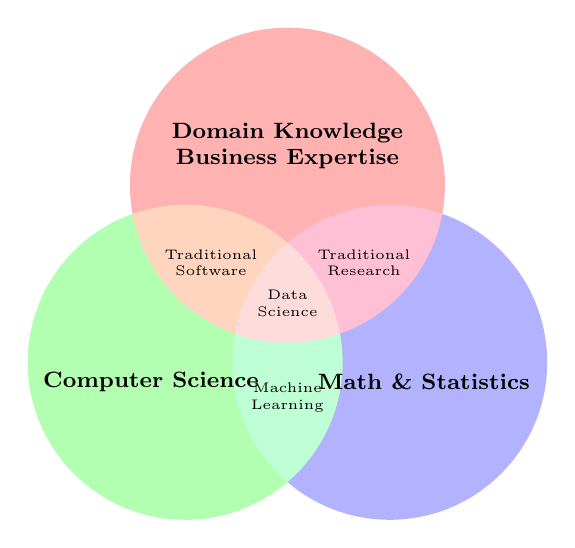
\begin{tikzpicture}
                            \begin{scope}[blend group=soft light]
                            \fill[red!30!white] (90:1.5) circle (2);
                            \fill[green!30!white] (210:1.5) circle (2);
                            \fill[blue!30!white] (330:1.5) circle (2);
                            \end{scope}
                            \node at (90:2) [font=\footnotesize, align=center]{\textbf{Domain Knowledge}\\\textbf{Business Expertise}};
                            \node at (210:2) [font=\footnotesize, align=center] {\textbf{Computer Science}};
                            \node at (330:2) [font=\footnotesize, align=center] {\textbf{Math \& Statistics}};
                            \node at (0:0) [font=\tiny, align=center] {Data\\Science};
                            \node at (28:1.1) [font=\tiny, align=center] {Traditional\\Research};
                            \node at (-28:-1.1) [font=\tiny, align=center] {Traditional\\Software};
                            \node at (90:-1.2) [font=\tiny, align=center] {Machine\\Learning};
                        \end{tikzpicture}
                    \end{adjustbox}
                \end{figure}
            \end{column}
        \end{columns}
    \end{frame}
    
    \begin{frame}{Terminology II/II}
        \begin{figure}
            \label{fig:data-scientist}
            \includegraphics[width=.7\textwidth]{figures/external/data-scientist.png}
            
            \textit{"The \textbf{data scientist role is critical for organizations} looking to \textbf{extract insight from information assets} for „big data“ initiatives and requires a \textbf{broad combination of skills} that may be fulfilled better as a team, for example: Collaboration and team work is required for working with business stakeholders to \textbf{understand business issues}. \textbf{Analytical and decision modeling skills} are required for discovering relationships within data and detecting patterns. \textbf{Data management skills} are required to build the relevant dataset used for the analysis."} - Gartner IT Glossary
        \end{figure}
    \end{frame}
    
    \begin{frame}{Business Intelligence versus Data Science}
        \begin{table}
            \scalebox{1}{
                {\RaggedRight
                    \begin{tabular}{m{2cm}m{5cm}m{5cm}}
                        \toprule
                        & \textbf{Business Intelligence} & \textbf{Data Science} \\
                        \midrule
                        \textbf{Perspective} & Looking backwards & Looking forwards \\
                        \textbf{Actions} & Slice and Dice & Interact \\
                        \textbf{Expertise} & Business User & Data Scientist \\
                        \textbf{Data} & Warehoused, Siloed & Distributed, real-time \\
                        \textbf{Scope} & Unlimited & Specific business question \\			
                        \textbf{Questions} & What happened? & What will happen? What if? \\
                        \textbf{Output} & Table & Answer \\
                        \textbf{Applicability} & Historic, possible confounding factors & Future, correcting for influences \\
                        \textbf{Tools} & SAP, Cognos, Microstrategy, SAS & Python, R, QlikView, Tableau \\
                        \textbf{Hot or not?} & So 1997 & Transformational \\
                        \bottomrule
                    \end{tabular}
                }
            }
        \end{table}
    \end{frame}
    
    \begin{frame}{Statistics versus Data Science}
        \begin{table}
            \scalebox{1}{
                {\RaggedRight
                    \begin{tabular}{m{2cm}m{5cm}m{5cm}}
                        \toprule
                        & \textbf{Statistics} & \textbf{Data Science} \\
                        \midrule
                        \textbf{Image} & Baseball (Cricket) & Sexiest Job of 21st Century \\
                        \textbf{Mode} & Reactive & Consultative \\
                        \textbf{Works} & Solo & In a team \\
                        \textbf{Inputs} & Data File, Hypothesis & A Business Problem \\
                        \textbf{Data} & Pre-prepared, clean & Distributed, messy, unstructured \\
                        \textbf{Data Size} & Kilobytes & Gigabytes \\			
                        \textbf{Tools} & SAS, Mainframe & R, Python, awk, Hadoop, Linux \\
                        \textbf{Nouns} & Tables & Data Visualizations \\
                        \textbf{Focus} & Inference (why) & Prediction (what) \\
                        \textbf{Output} & Report & Data App / Data Product \\
                        \textbf{Latency} & Weeks & Seconds \\
                        \bottomrule
                    \end{tabular}
                }
            }
        \end{table}
    \end{frame}
    
    \begin{frame}{Data Analytics Types}
        \begin{columns}
            \begin{column}{.6\textwidth}
                \begin{justify}
                    \alert{\textbf{\textsc{Descriptive analytics}}}
                    
                    Descriptive analytics answers the question of \textbf{what is happening now} and \textbf{what has happened in the past}. It is only able to reveal that something went wrong or right but \textbf{without explaining why}.
                    \vspace*{2mm}
                    
                    \alert{\textbf{\textsc{Diagnostic analytics}}}
                    
                    In diagnostic analytics, \textbf{historical data} is used to \textbf{discover or to determine why something happened}. It allows to find out \textbf{dependencies} and to \textbf{identify patterns}.
                    
                    \vspace*{2mm}
                    
                    \alert{\textbf{\textsc{Predictive analytics}}}
                    
                    Predictive analytics uses the \textbf{findings of descriptive and diagnostic analytics} to detect \textbf{tendencies, clusters and exceptions} in order to \textbf{predict the future} which in turn makes it a \textbf{tool for forecasting}. 
                    
                    \vspace*{2mm}
                    
                    \alert{\textbf{\textsc{Prescriptive analytics}}}
                    
                    The purpose of prescriptive analytics is to reveal \textbf{what actions should be taken} in order to eliminate a \textbf{future problem} or to \textbf{take full advantage of a promising trend}. This kind of analysis often results in \textbf{rules} and \textbf{recommendations}.
                \end{justify}
            \end{column}
            \begin{column}{.4\textwidth}
                \begin{figure}
                    \label{fig:data-analytics-types}
                    \includegraphics[width=.9\textwidth]{figures/external/data-analytics-types.png}
                \end{figure}
            \end{column}
        \end{columns}
    \end{frame}
    
    \begin{frame}{Data Analytics Value Chain}
        \begin{figure}
            \label{fig:data-analytics-value-chain}
            \includegraphics[width=\textwidth]{figures/external/analytics-value-chain.png}
        \end{figure}
    \end{frame}
    
    \begin{frame}{Cross-Industry Standard Process for Data Mining I/II}
        \begin{columns}
            \begin{column}{.6\textwidth}
                \begin{justify}
                    \alert{\textbf{\textsc{Business understanding}}}
                    
                    Understanding the \textbf{project objectives and requirements from a business perspective}, then converting this knowledge into a \textbf{data mining problem definition}.
                    \vspace*{2mm}
                    
                    \alert{\textbf{\textsc{Data understanding}}}
                    
                    Collecting data and proceeding with activities to get familiar with the dataset by \textbf{describing, exploring and verifying} it in order to\textbf{ discover an initial level of insights} or to \textbf{detect interesting subsets to form hypotheses} for hidden information.
                    \vspace*{2mm}
                    
                    \alert{\textbf{\textsc{Data preparation}}}
                    
                    Constructing the \textbf{final analytical dataset from initial raw data by selection, transformation and cleaning}. Performed multiple times and not in any prescribed order. Quality of cleaned data will have an impact on model performance.
                \end{justify}
            \end{column}
            \begin{column}{.4\textwidth}
                \begin{figure}
                    \label{fig:crisp-1}
                    \includegraphics[width=.9\textwidth]{figures/external/crisp.png}
                \end{figure}
            \end{column}
        \end{columns}
    \end{frame}
    
    \begin{frame}{Cross-Industry Standard Process for Data Mining II/II}
        \begin{columns}
            \begin{column}{.6\textwidth}
                \begin{justify}
                    \alert{\textbf{\textsc{Modeling}}}
                    
                    \textbf{Selecting and applying various modeling techniques} and calibrating their parameters to optimal values. As some \textbf{techniques have specific requirements} on the form of data, \textbf{stepping back to the data preparation phase} is often necessary.
                    \vspace*{2mm}
                    
                    \alert{\textbf{\textsc{Evaluation}}}
                    
                    Evaluating the model and reviewing the steps executed to construct the model to be certain it properly achieves the business objectives and to decide whether or not to use the results in production.                
                    \vspace*{2mm}
                    
                    \alert{\textbf{\textsc{Deployment}}}
                    
                    Determining how to\textbf{ utilize the results} and how to \textbf{organize and present the knowledge} gained to customers in a way that they can use it. Can be a \textbf{simple report} or a \textbf{complex data application}.
                \end{justify}
            \end{column}
            \begin{column}{.4\textwidth}
                \begin{figure}
                    \label{fig:crisp-2}
                    \includegraphics[width=.9\textwidth]{figures/external/crisp.png}
                \end{figure}
            \end{column}
        \end{columns}
    \end{frame}

    \subsection{Basic Statistics Refresher}
    
    \begin{frame}{Dataset Anatomy}
        \begin{figure}
            \label{fig:dataset-anatomy}
            \includegraphics[width=\textwidth]{figures/external/dataset-anatomy.pdf}
        \end{figure}
    \end{frame}

    \begin{frame}{Common Variable Types}
        \begin{columns}
            \begin{column}[t]{.45\textwidth}
                \begin{justify}
                    \alert{\textbf{\textsc{Qualitative variable}}}
                    
                    Qualitative variables, also called \textbf{categorical variables}, take on values that are \textbf{names or labels}, e.g., the gender.
                \end{justify}
            \end{column}
            \begin{column}[t]{.45\textwidth}
                \begin{justify}
                    \alert{\textbf{\textsc{Quantitative variable}}}
                    
                    Quantitative variables are numeric and \textbf{represent a measurable quantity}, e.g., the number of people in a city.
                \end{justify}
            \end{column}
        \end{columns}
    
        \begin{columns}
            \begin{column}[t]{.45\textwidth}
                \begin{justify}
                    \alert{\textbf{\textsc{Discrete variable}}}
                    
                    Discrete variables can only take on a \textbf{finite number of values}, e.g., the number of cars owned.
                \end{justify}
            \end{column}
            \begin{column}[t]{.45\textwidth}
                \begin{justify}
                    \alert{\textbf{\textsc{Continuous variable}}}
                    
                    Continuous variables can take on \textbf{any value in a certain range}, e.g., the body height.
                \end{justify}
            \end{column}
        \end{columns}
    \end{frame}

    \begin{frame}{Measurement Scales}
        \begin{columns}
            \begin{column}[t]{.45\textwidth}
                \begin{justify}
                    \alert{\textbf{\textsc{Nominal scale}}}
                    
                    Characteristic attributes can be \textbf{distinguished}, e.g., gender. A subtype of nominal scale with only two categories (e.g. male/female) is called \textbf{dichotomous}. 
                    \vspace*{4mm}
                    
                    \alert{\textbf{\textsc{Ordinal scale}}}
                    
                    Characteristic attributes can be \textbf{distinguished} and \textbf{ranked}, e.g., educational achievement. However, intervals between the values can neither be \textbf{compared} nor \textbf{interpreted}.
                \end{justify}
            \end{column}
            \begin{column}[t]{.45\textwidth}
                \begin{justify}
                    \alert{\textbf{\textsc{Metric scale}}}
                    
                    Characteristic attributes can be \textbf{distinguished} and \textbf{ranked}. The intervals between then can be \textbf{compared}. The metric scale further divides into the \textbf{interval scale} and the \textbf{ratio scale}. The ratio scale has a \textbf{naturally given point of origin} (e.g., body weight), whereas the interval scale has an \textbf{artificially given point of origin} (e.g., calculation of times).
                \end{justify}
            \end{column}
        \end{columns}
    \end{frame}	

    \stepcounter{openexercise}
    \begin{frame}{Open Exercise \arabic{openexercise}}
        For each of the following features below state whether it is qualitative or quantitative and whether it is discrete or continuous. Also state its measurement scale.
        
        \begin{enumerate}[a)]
            \item Postal code (e.g., 42119)
            \item Income group (e.g., < \$20,000, \$20,000-\$40,000, > \$40,000)
            \item Body height (e.g., 189cm)
            \item Temperature in degree Centigrade (e.g., 20°C)
        \end{enumerate}
    \end{frame}	

    \note[itemize]
    {
        \item[a)]{Qualitative, discrete, nominal scale}
        \item[b)]{Qualitative, discrete, ordinal scale}
        \item[c)]{Quantitative, metric, ratio scale}
        \item[d)]{Quantitative, metric, interval scale}
    }
\end{document}